\subsubsection{Gl{\"u}ck} \label{glueck-1}



\todo[inline,color=green!40]{Verantwortlich: Minas\\
- RfP}



Das Wort ``Gl{\"u}ck'' wird im deutschsprachigen Gebrauch mit zwei unterschiedlichen Grundbedeutungen verwendet. 
In anderen Sprachen wird dieser Begriff auseinandergehalten z.B. im englischen als ``luck'' und ``happiness'' und im franz{\"o}sichen als ``la bonne chance'' und ``le bonbeur''.
Im deutschen Sprachgebrauch muss zwischen den Gl{\"u}ckszufall und die Gl{\"u}cksgabe, welches nicht erzwungen werden kann und zwischen das Gl{\"u}cklichsein, die Gl{\"u}ckserfahrung und das Gl{\"u}ckserlebnis unterschieden werden\cite{bien19}. \\

In diesem Szenario war es die Absicht anhand Fotos mit Texten und Musik im Hintergrund eine Gl{\"u}ckserfahrung oder auch ein Gl{\"u}ckserlebnis bei den Probanden auszul{\"o}sen.
Abbildung \ref{fig-glueck} zeigt die hierf{\"u}r verwendeten Bilder und deren Texte. \\

\begin{figure}[H] \centering
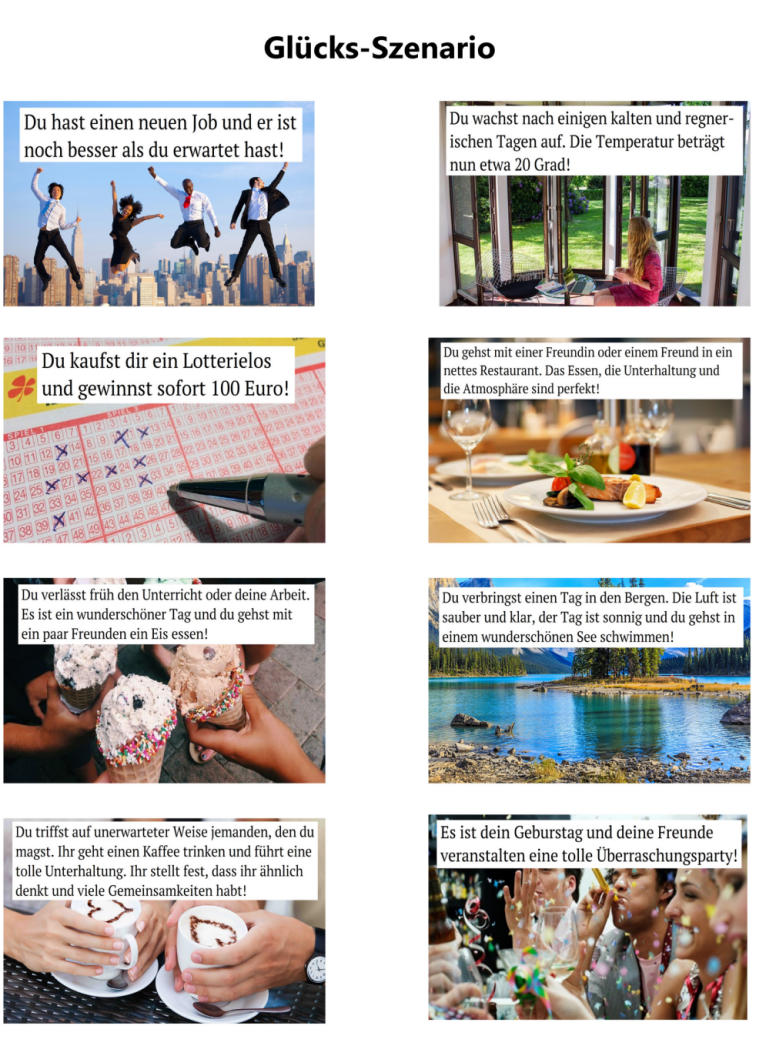
\includegraphics[width=12cm]{Images/gluck.png} 
\vspace{-0.3cm} 
\caption{Vignetten f{\"u}r das Gl{\"u}cks-Szenario.}
\label{fig-glueck} 
\end{figure}

Die Bilder wurden in einer PowerPoint-Pr{\"a}sentation abgespielt. 
Diese wechselten alle 30 Sekunden, w{\"a}hrend die Audiodatei im Hintergrund ablief.
Die Idee stammt von der wissenschaftlichen Publikation ``Mood inductions for four specific moods: A procedure employing guided imagery vignettes with music,'' von J. D. Mayer, J. P. Allen, und K. Beauregard. 
In dieser Publikation wurde versucht anhand Vignetten und Hintergrundmusik Gl{\"u}cksemotionen auszul{\"o}sen.
Die verwendete Audiodatei aus der Publikation, welches aus dem Ballettst{\"u}ck ``Coppélia ou La Fille aux yeux d'émail'' stammte, wurde in diesem Szenario {\"u}bernommen. 
Die aus der Publikation verwendeten Vignetten wurden insofern modifiziert, das einzelne durch eigene Vignetten ersetzt wurden.

